\section{Auswertung}
\label{sec:Auswertung}

Alle Berechnungen werden mit dem Programm \glqq Numpy" \cite{numpy}, die Unsicherheiten mit dem Modul \glqq Uncertainties" \cite{uncertainties}, die Ausgleichsrechnungen mit dem Modul \glqq Scipy" \cite{scipy} durchgeführt und die grafischen Darstellungen über das Modul \glqq Matplotlib" \cite{matplotlib} erstellt.

\subsection{Untergrundrate}

Aus dem mehrfachen Messen der Untergrundrate ergeben sich die Messwerte $N_U=\{ 129, 143, 144, 136, 139, 126, 158 \}$. Aus diesen Messwerten wird der Mittelwert berechnet. Dieser ergibt sich zu $\num{139(4)}$. Da die Zeit, über die die Impulse gemessen werden, mit den Messintervallen der folgenden Messergebnisse übereinstimmen muss, wird  dieser Mittelwert auf die jeweiligen Messintervalle skaliert. So ergibt sich eine Untergrundrate von $N_{U_V}=\num{14(1)}$ in einem Zeitintervall von $\Delta t=\SI{30}{\s}$ und $N_{U_R}=\num{7(1)}$ in einem Zeitintervall von $\Delta t=\SI{15}{\s}$.

\subsection{Halbertszeit Vanadium}

Die gemessenen Impulse sind in Tablle \ref{tab:V} aufgeführt. Von den gemessenen Impulsmengen muss gemäß Gleichung REFFFFFFFFFFFFF jeweils die Untergrundrate $N_{U_R}$ abgezogen werden. Die dadurch bestimmten Impulsraten sind grafisch in einem Halblogarhythmischen Diagramm REFFFFFFFF dargestellt. Über Gleichung REFFFFFF lässt sich ein linearer Zusmmenhang zwischen $\ln{N}$ und der Zerfallskonstante $\lambda $ feststellen. Wird also eine lineare Regression durchgeführt, so ergibt sich eine Gerade
\begin{equation}
    \ln{N}(t)=a*t + b
\end{equation}
mit den Geradenparametern $a=$ und $b=$. 

\begin{table}
\centering
\caption{Anzahl registrierter Impulse der Vanadium-Probe.}
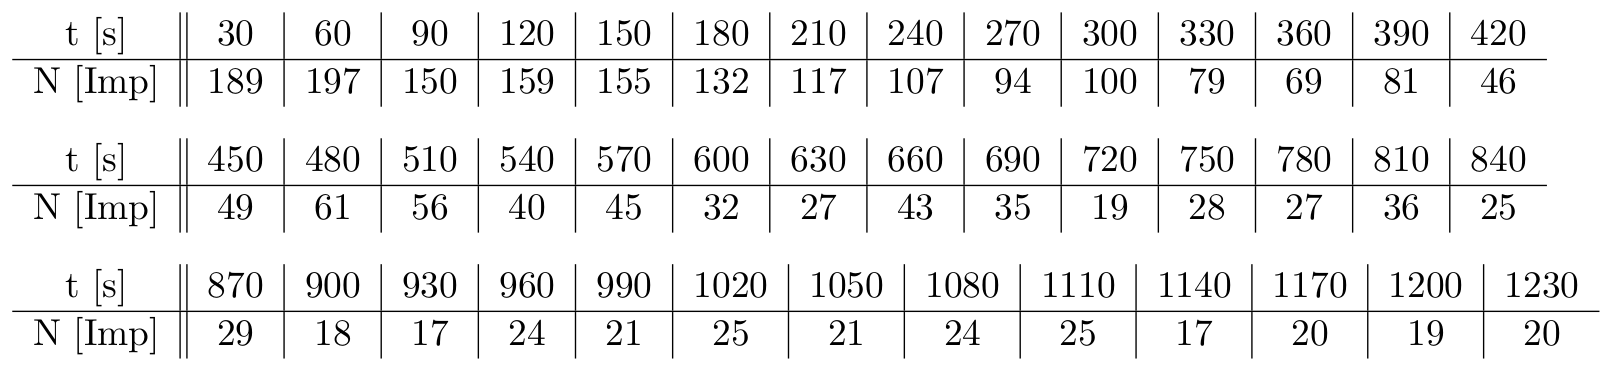
\includegraphics[width=\textwidth]{data/Vanadium.png}
\label{tab:V}
\end{table}


\subsection{Halbertszeit Rhodium}
\begin{table}
\centering
\caption{Anzahl registrierter Impulse der Rhodium-Probe.}
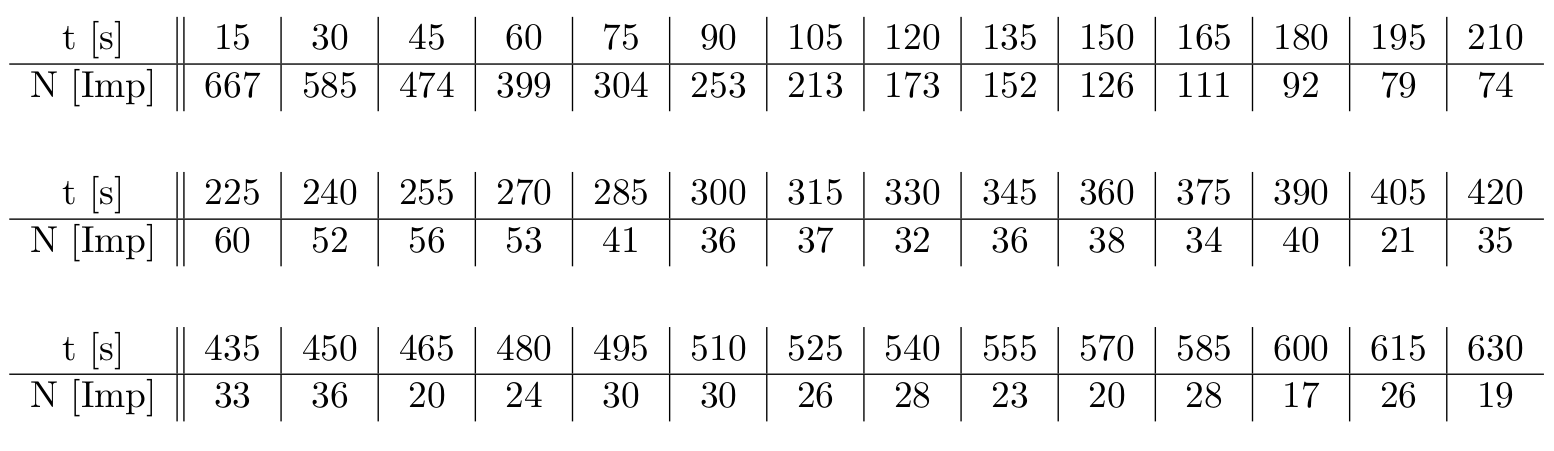
\includegraphics[width=\textwidth]{data/Rhodium.png}
\label{tab:R}
\end{table}


%Messwerte: Alle gemessenen physikalischen Größen sind übersichtlich darzustellen.
%
%Auswertung:
%Berechnung der geforderten Endergebnisse
%mit allen Zwischenrechnungen und Fehlerformeln, sodass die Rechnung nachvollziehbar ist.
%Eine kurze Erläuterung der Rechnungen (z.B. verwendete Programme)
%Graphische Darstellung der Ergebnisse